\documentclass[journal]{IEEEtran}
\usepackage[utf8]{inputenc}

%\usepackage[retainorgcmds]{IEEEtrantools}
% \usepackage{bibentry}  
\usepackage{xcolor,soul,framed} %,caption

\colorlet{shadecolor}{yellow}
% \usepackage{color,soul}
\usepackage[pdftex]{graphicx}
\usepackage{grffile}
\graphicspath{{../pdf/}{../jpeg/}}
\DeclareGraphicsExtensions{.pdf,.jpeg,.png}

\usepackage[cmex10]{amsmath}
\usepackage{amssymb}
%Mathabx do not work on ScribTex => Removed
%\usepackage{mathabx}
\usepackage{array}
\usepackage{mdwmath}
\usepackage{mdwtab}
\usepackage{eqparbox}
\usepackage{url}

% \usepackage{hyperref}

\usepackage{float}
\usepackage{listings}

%\bstctlcite{IEEE:BSTcontrol}
\newcommand{\R}{\mathbb{R}}

%=== TITLE & AUTHORS ====================================================================
\begin{document}
  \title{TP2 - Ant Colony Optimization (ACO)\\
  Longest Path} 
  \author{Yuri Niitsuma}

\maketitle

% \input{chapters/abstract.tex}
\section{Introdução}

O objetivo desse trabalho é desenvolver conceitos chaves para construções de soluções para
problemas usando Ant Colony Optimization (ACO), envolvendo o entendimento e a implementação
dos componentes básicos de um arcabouço de ACO, bem como a análise de sensibilidade dos seus
parâmetros (como eles afetam o resultado final, a natureza de convergência,
etc) e procedimentos para avaliação das soluções alcançadas. Para esse trabalho, vocês devem
elaborar soluções para o problema conhecido como \textbf{longest path problem}.

Dado um grafo $G(V, E)$, uma função $w : E \rightarrow R$ que atribui pesos a cada aresta e dois vértices $u, v \in V$ ,
denotaremos como $\mathcal{P}$ o conjunto de caminhos simples partindo de $u$ e chegando em $v$.
O problema consiste então em encontrar
$P^* = \{e_1^*, e_2^*, \dots, e_k^*\}$
tal que

$$P^* = \arg \max\limits_{P \in \mathcal{P}} \sum\limits_{e_i \in P} w(e_i)$$

Ou seja, queremos encontrar o caminho simples de $u$ a $v$ que maximize o peso total do
caminho.

\section{Implementação}

O ACO foi modelado utilizando as principais bibliotecas:

\begin{itemize}
	\item \textbf{numpy}
	\item \textbf{networkx}: biblioteca para grafos
\end{itemize}

As bibliotecas instaladas, via \textbf{pip}, pelo \textbf{virtual-env} encontra-se
no arquivo \textbf{req.txt}.

\subsection{Grafo}

Seja o grafo $G(V, E)$, definimos baseado na especificação.

\begin{itemize}
	\item O grafo $G$ é direcionado.
	\item Cara aresta do grafo contém, como atributo, pesos dados como entrada, a taxa de feromônio $t_{xy}$ e a probabilidade
	da formiga escolher a aresta $p_{xy}$ que é atualizado no final de cada iteração. Sendo $xy$ a direção da aresta do nó $x$ a $y$.
	\item Como o custo de encontrar um caminho entre os nós $u$ e $v$ é caro, assumimos que existe um caminho simples. Caso contrário,
	entrará em loop infinito. Isto não acontece com os \textit{datasets} \textbf{graph1}, \textbf{graph2} e \textbf{graph3}.
\end{itemize}

\subsection{Fluxo}

a iteração fica  
encontrar caminho das formigas  
armazenar os valores dos feromonios  
update pheromone  
evaporate pheromones  

INSERIR DESENHO

\subsection{Atualização Feromônio}

% self[u][v]['t_xy'] += (ant.fitness + 0.5 - ant.pheromone[i][2]) / max_pher
%                 # self[u][v]['t_xy'] += 1.0 - 1.0 / ant.fitness
% 								self[u][v]['t_xy'] = min(self[u][v]['t_xy'], 100.0)



$$t_{xy} \leftarrow \frac{fitness_k - pheromone_{xy} + 0.5}{\max \forall fitness}$$

Assim o feromônio é mais forte no início do caminho e fica mais fraco ao final. Isto ajuda
a criar mais caminhos com o prefixo do melhor caminho e tentar variar nas arestas posteriores.

\section{Experimentos}

A princípio foram testados variações dos parâmetros de \textit{crossover} e \textit{mutação} mantendo constante outros parâmetros. Os erros gerados no gráfico é a média da média da fitness dos indivíduos por geração em 15 instâncias de testes.

Nos gráficos, o último erro médio da geração 50 é a base de dados de teste. Percebe-se que este erro quase sempre está acima do erro do treinamento pela maldição do \textit{overfitting}.

\subsection{Crossover}

Não se percebe um impacto grande na convergência, pois depende da variabilidade da população inicial para o cruzamento encontrar novos indivíduos que contenham fitness melhores. Por exemplo, se a base de dados tiver um comportamento senoidal e nenhum indivíduo tiver uma sub-árvore que contenha seno ou cosseno. Nenhum cruzamento gerará um nó trigonométrico que diminuirá o erro.

\begin{figure}[H]
  \centering
  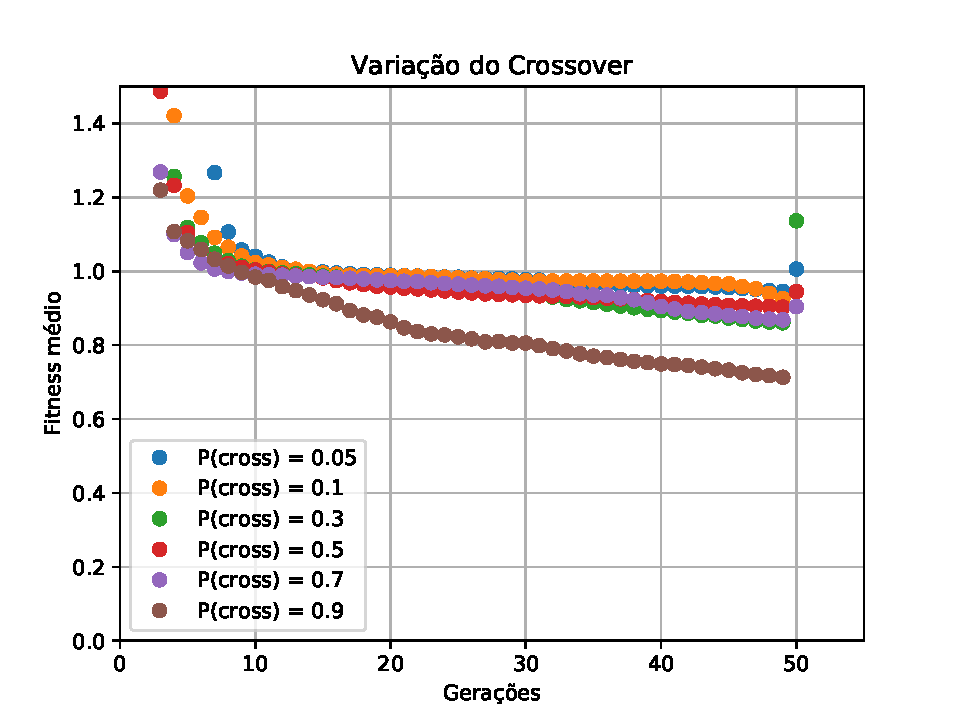
\includegraphics[width=0.5\textwidth]{pdf/varcrossover.pdf}
  \label{fig:varcross}
\end{figure}

\subsection{Mutação}

Na mutação percebemos que a convergência possui maior efeito, pois a mutação torna-se maior a variabilidade da população que probabilisticamente possui chances de algum nó gerado melhorar a fitness no treinamento.

\begin{figure}[H]
  \centering
  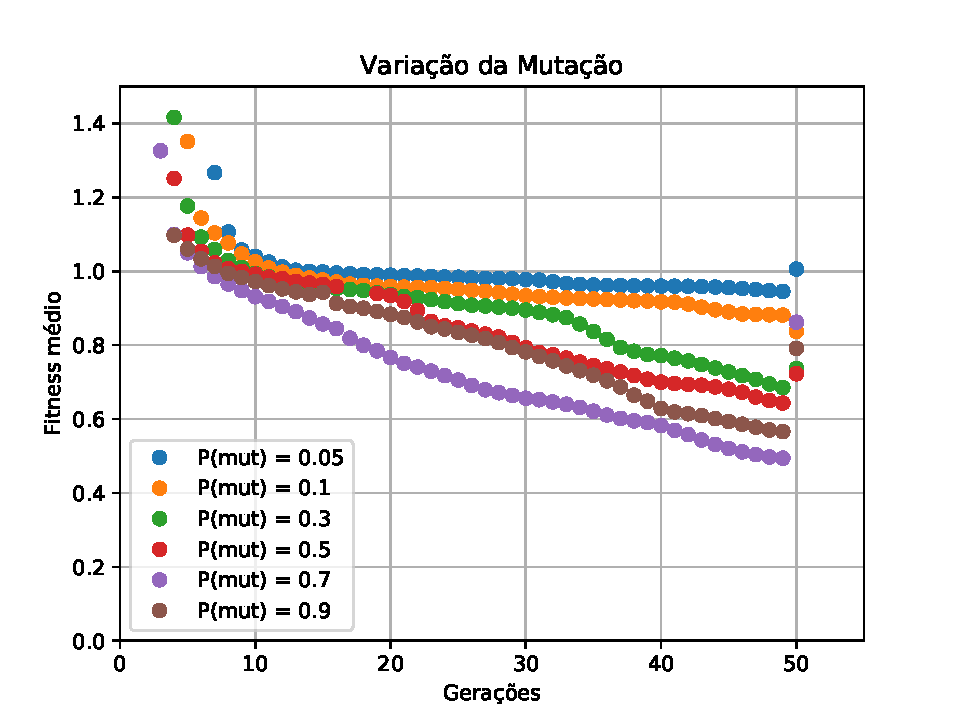
\includegraphics[width=0.5\textwidth]{pdf/varmutation.pdf}
  \label{fig:varmut}
\end{figure}

\subsection{Torneio}

O torneio percebe-se que possui uma maior pressão a convergência, mas em contra-partida diminui a variabilidade, pois em vários torneios o melhor indivíduo da população pode ser escolhido várias vezes.

\begin{figure}[H]
  \centering
  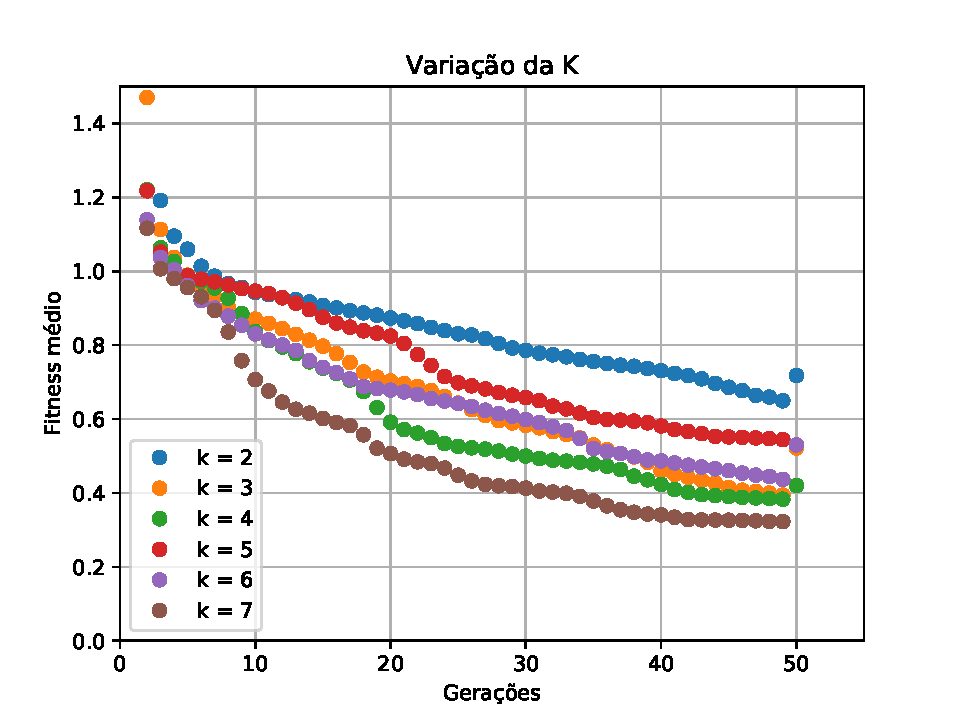
\includegraphics[width=0.5\textwidth]{pdf/varK.pdf}
  \label{fig:vark}
\end{figure}

\subsection{População}

A variação da quantidade da população impacta na variabilidade que ocasiona na probabilidade de gerar novos invivíduos diferentes. Com a convergência, observa-se que após a convergência não há mais variabilidade e a fitness e tende a permanecer constante pois não há nenhum método de \textit{niching}.

\begin{figure}[H]
  \centering
  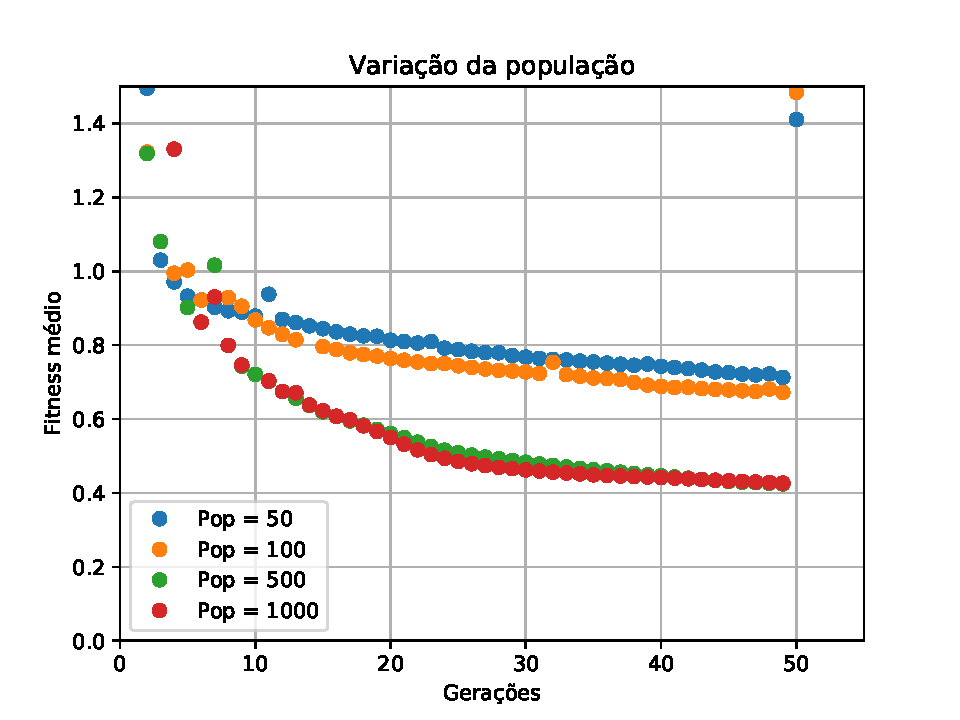
\includegraphics[width=0.5\textwidth]{pdf/populations.pdf}
  \label{fig:varpop}
\end{figure}




% • Escolher o tamanho da popula ̧c ̃ao e o nu ́mero de gerac ̧ ̃oes apropriados. O tamanho da popula ̧c ̃ao pode ser testado, por exemplo, utilizando 50, 100, 500 indiv ́ıduos. O nu ́mero de gera ̧c ̃oes pode tamb ́em ser escolhido usando esses mesmos nu ́meros. Mas como saber se o escolhido  ́e o mais apropriado? Vocˆe pode avaliar como o aumento no nu ́mero da popula ̧c ̃ao ou de gerac ̧ ̃oes melhora a soluc ̧ ̃ao encontrada (em termos do erro gerado), se a popula ̧c ̃ao converge, etc.
% • Testar duas configura ̧c ̃oes de parˆametros para cruzamento e muta ̧c ̃ao. Na primeira, a probabilidade de cruzamento (pc) deve ser alta (por exemplo, 0.9), e a probabilidade de muta ̧c ̃ao (pm) deve ser baixa (por exemplo, 0.05). Na segunda, pc deve ser mais baixa (por exemplo, 0.6) e pm mais alta (por exemplo, 0.3). Para ambas as configura ̧c ̃oes, deve-se avaliar o efeito do cruzamento e da muta ̧c ̃ao na evolu ̧c ̃ao, isto  ́e, em quantos casos esses operadores contribuem positivamente (os filhos gerados s ̃ao melhores que os pais) ou negativamente para a evolu ̧c ̃ao? A partir desse estudo inicial, que valores finais vocˆe proporia?
% • Analisar as mudan ̧cas ocorridas quando o tamanho do torneio aumenta de 2 para 5 ou 3 para 7, dependendo do tamanho inicial da popula ̧c ̃ao.
% • Analisar o impacto de usar somente operadores elitistas.
% • Existe uma forma simples de medir bloating no seu algoritmo?

\section{Conclusão}

Este trabalho mostrou as capacidades do algoritmo heurístico ACO para encontrar boas soluções
do problema \textit{longest path problem}. Mostrou-se também o impacto de alguns dos seus parâmetros
no algoritmo e as características de seus grafos.

\section{Referências}

Ant colony optimization: a new meta-heuristic \textit{Dorigo, Marco and Di Caro, Gianni}


\bibliography{ref}

\end{document}


